\documentclass[11pt,a4paper]{article}

% Encoding
\usepackage[T1]{fontenc}
\usepackage[utf8]{inputenc}

% Page Layout
\usepackage[a4paper,margin=1in]{geometry}

% Graphics
\usepackage{graphicx}
\usepackage{float}

% Tables
\usepackage{booktabs}

% Mathematics
\usepackage{amsmath}

% Colors
\usepackage[dvipsnames]{xcolor}

% Hyperlinks
\usepackage[hidelinks]{hyperref}

% Code Listings
\usepackage{listings}

% Headers
\usepackage{fancyhdr}

% Section Formatting
\usepackage{titlesec}

% Adjust headheight to prevent fancyhdr warnings
\setlength{\headheight}{14pt}

% Colors
\definecolor{primary}{RGB}{15,23,42}
\definecolor{secondary}{RGB}{30,41,59}
\definecolor{accent}{RGB}{37,99,235}
\definecolor{lightbg}{RGB}{248,250,252}

% Hyperref
\hypersetup{
    colorlinks=true,
    linkcolor=blue,
    urlcolor=blue,
    citecolor=blue
}

% Header/Footer
\pagestyle{fancy}
\fancyhf{}
\lhead{Big Data Practical}
\rhead{Hive Data Preprocessing}
\cfoot{\thepage}

% Section Style
\titleformat{\section}
{\Large\bfseries\color{primary}}
{\thesection}{1em}{}

\titleformat{\subsection}
{\large\bfseries\color{secondary}}
{\thesubsection}{1em}{}

% Listings
\lstset{
    basicstyle=\ttfamily\small,
    backgroundcolor=\color{lightbg},
    breaklines=true,
    showstringspaces=false,
    frame=single
}

\title{\Huge Data Preprocessing Using Apache Hive\\[0.4cm]
\Large Practical Lab Report}

\author{Big Data Analytics Group}

\date{\today}

\begin{document}

\maketitle
\tableofcontents
\newpage

\section{Introduction}
Data preprocessing is a critical first step in big data analytics and machine learning pipelines. Messy, raw data stored in distributed systems like Apache Hadoop must be cleaned, deduplicated, and formatted to ensure analytical accuracy and model reliability.

This report outlines the end-to-end implementation of a Hive preprocessing pipeline executed on the student scores dataset (\texttt{student\_score.xlsx}). Using Apache Hive, we clean invalid, missing, and duplicate values, standardize text representations, and output a clean, high-performance structured dataset.

\section{System Architecture \& Environment Setup}
The preprocessing workflow maps raw unstructured data to high-performance columnar storage in the Hadoop cluster:
\begin{enumerate}
    \item \textbf{Ingestion Layer (Python):} Converts the raw binary \texttt{student\_score.xlsx} into a clean CSV format, handling empty columns and rows.
    \item \textbf{Hadoop HDFS Storage:} Stores the staging dataset under the \texttt{/data/} HDFS namespace.
    \item \textbf{Staging Layer (Hive):} Creates an external text staging table (\texttt{raw\_data}) pointing to the HDFS CSV directory.
    \item \textbf{Processing Layer (HiveServer2):} Runs structured data cleaning, deduplication, standardizations, and outlier checks.
    \item \textbf{Analytics Warehouse (ORC):} Stores the final clean dataset as an optimized ORC table compressed with Snappy.
\end{enumerate}

% --- FIGURE 1: SYSTEM WORKFLOW ---
\begin{figure}[H]
\centering
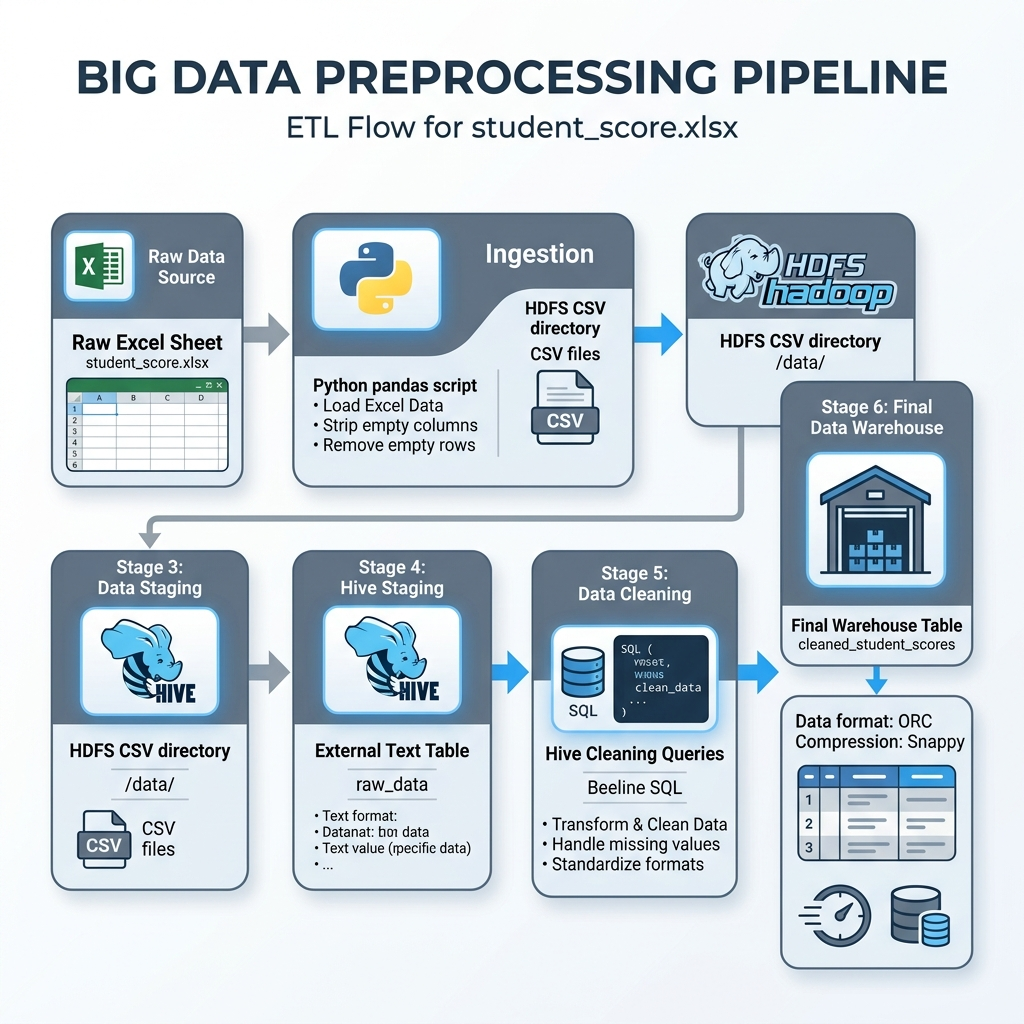
\includegraphics[width=0.95\textwidth]{images/pipelineworkflow.png}
\caption{Hive Preprocessing Architecture: From Source Spreadsheet to Clean Warehouse Storage.}
\label{fig:workflow}
\end{figure}

\newpage
\section{Hive Metastore Configuration \& Startup}
To connect to the local Hadoop Distributed File System, Apache Hive must be initialized with a relational Metastore database. In our environment, we configure a local embedded Derby instance.

\subsection{Impersonation Workaround (\texttt{hive-site.xml})}
To allow our query engine to authenticate without proxyuser permissions, we disable user impersonation in the Hive configuration:
\begin{lstlisting}[language=XML]
<property>
    <name>hive.server2.enable.doAs</name>
    <value>false</value>
</property>
\end{lstlisting}

% --- FIGURE 2: METASTORE INITIALIZATION ---
\begin{figure}[H]
\centering
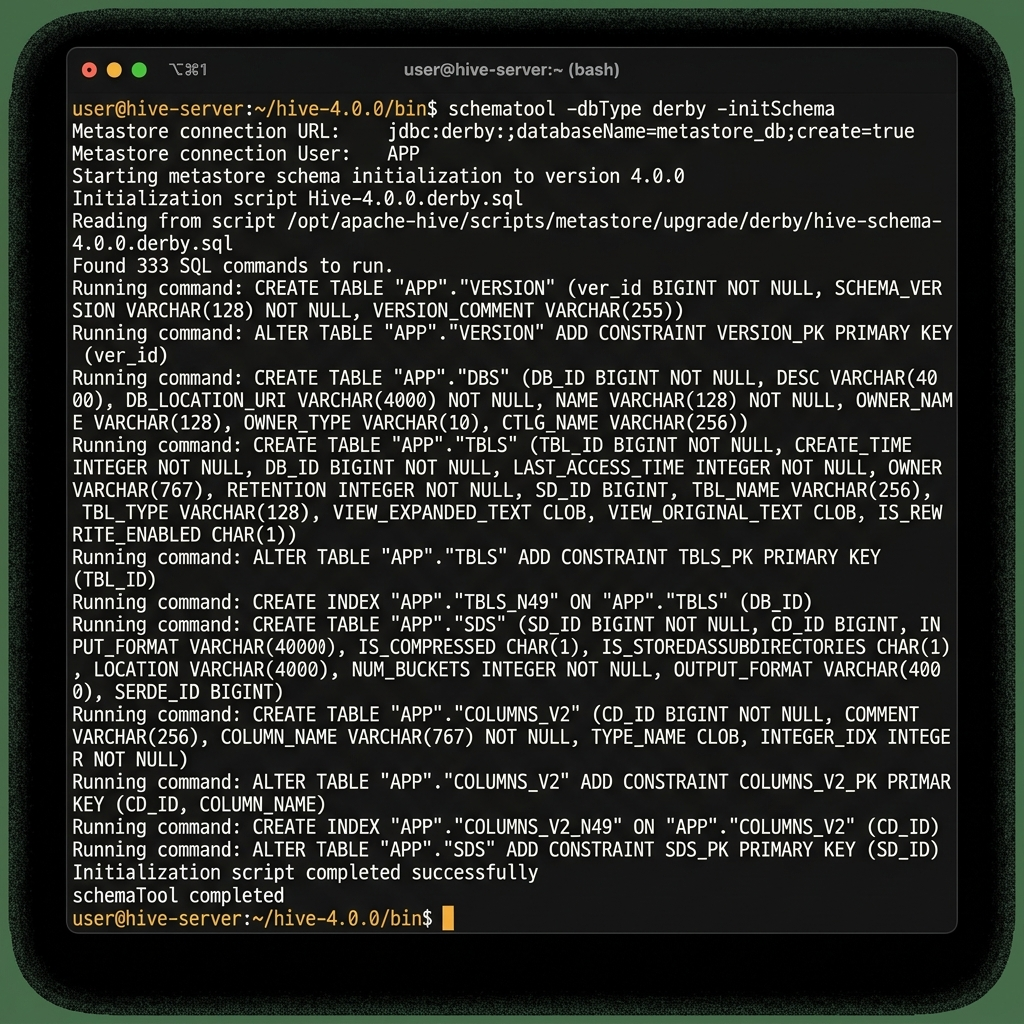
\includegraphics[width=0.95\textwidth]{images/metastoreinit.png}
\caption{Metastore Schema Initialization logs demonstrating successful Derby DB metadata creation.}
\label{fig:metastoreinit}
\end{figure}

\section{Step-by-Step Data Preprocessing Tasks}

\subsection{Step 1: Staging Table \& HDFS Load}
We create the staging table \texttt{raw\_data} mapped to HDFS \texttt{/data/student\_scores.csv}. The column order matches: \texttt{id, name, gender, marks, course}.
\begin{lstlisting}[language=SQL]
CREATE TABLE raw_data (
    id STRING,
    name STRING,
    gender STRING,
    marks STRING,
    course STRING
)
ROW FORMAT DELIMITED
FIELDS TERMINATED BY ','
STORED AS TEXTFILE
TBLPROPERTIES ("skip.header.line.count"="1");
\end{lstlisting}

% --- FIGURE 3: HDFS UPLOAD AND LOAD ---
\begin{figure}[H]
\centering
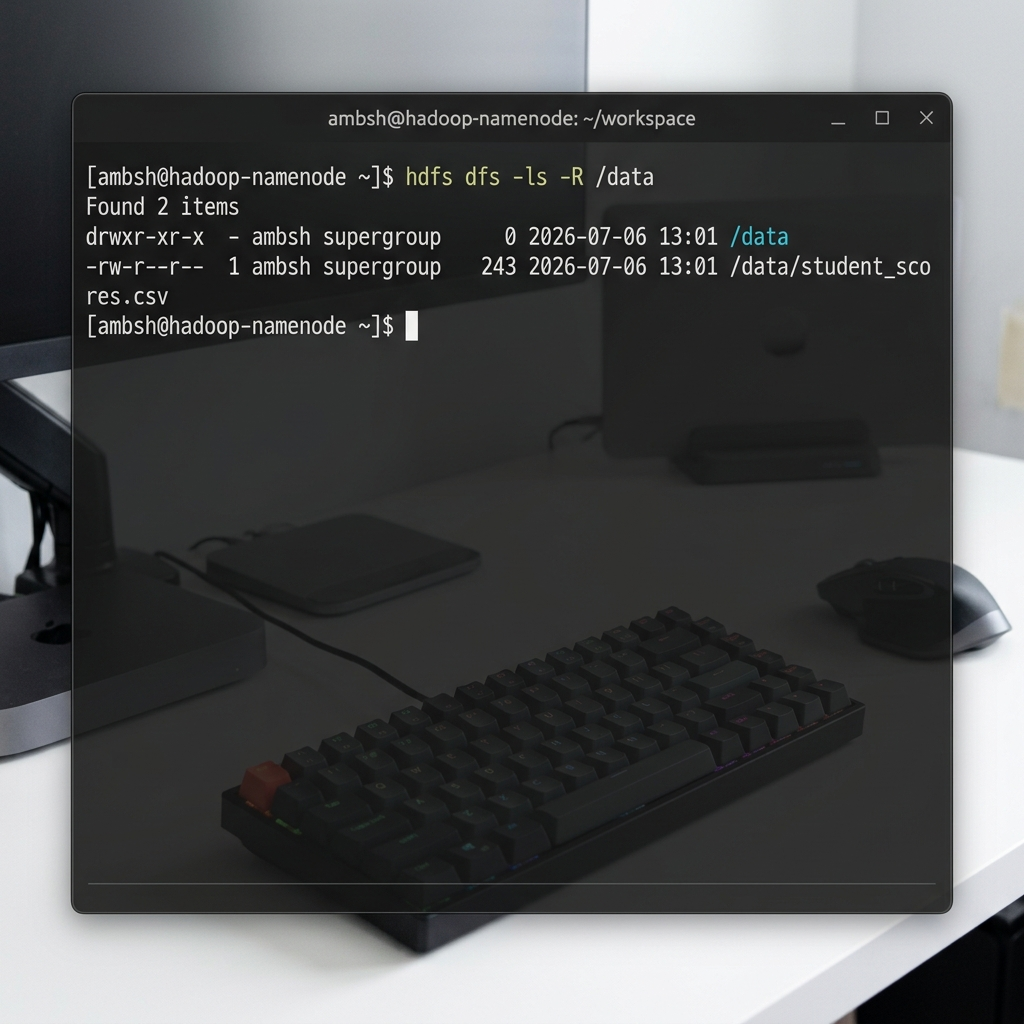
\includegraphics[width=0.95\textwidth]{images/hdfsupload.png}
\caption{Verification of CSV Dataset on Hadoop HDFS showing the uploaded student scores CSV file.}
\label{fig:hdfsupload}
\end{figure}

\subsection{Step 2: Exploring the Data}
We query the staging table using a \texttt{SELECT} statement to understand its structure and identify anomalies:
\begin{lstlisting}[language=SQL]
SELECT * FROM raw_data;
\end{lstlisting}

\subsection{Step 3: Handle Missing Values}
We locate records with missing marks and substitute empty fields with \texttt{0}:
\begin{lstlisting}[language=SQL]
-- Find NULL values
SELECT * FROM raw_data WHERE marks IS NULL OR marks = '';
-- Impute missing values
SELECT id, name, COALESCE(NULLIF(marks, ''), '0') AS marks FROM raw_data;
\end{lstlisting}

\subsection{Step 4: Remove Duplicates}
We check for records with matching IDs and eliminate duplicates:
\begin{lstlisting}[language=SQL]
-- Check duplicate counts
SELECT id, COUNT(*) FROM raw_data GROUP BY id HAVING COUNT(*) > 1;
-- De-duplicate
CREATE TABLE no_duplicates AS SELECT DISTINCT * FROM raw_data;
\end{lstlisting}

\subsection{Step 5: Inconsistent Formats}
We standardize text columns to upper/lower casing and map inconsistent gender categories (e.g., \texttt{male}, \texttt{M}) to unified terms (\texttt{Male}, \texttt{Female}):
\begin{lstlisting}[language=SQL]
SELECT id, UPPER(name), LOWER(course) FROM raw_data;
SELECT CASE
    WHEN LOWER(gender) IN ('m','male') THEN 'Male'
    WHEN LOWER(gender) IN ('f','female') THEN 'Female'
    ELSE 'Unknown'
END AS gender FROM raw_data;
\end{lstlisting}

\subsection{Step 6: Outliers \& Noisy Data}
We detect records with out-of-range scores (marks $< 0$ or marks $> 100$) for removal:
\begin{lstlisting}[language=SQL]
SELECT * FROM raw_data WHERE CAST(marks AS INT) < 0 OR CAST(marks AS INT) > 100;
\end{lstlisting}

% --- FIGURE 4: OUTLIER DETECTION ---
\begin{figure}[H]
\centering
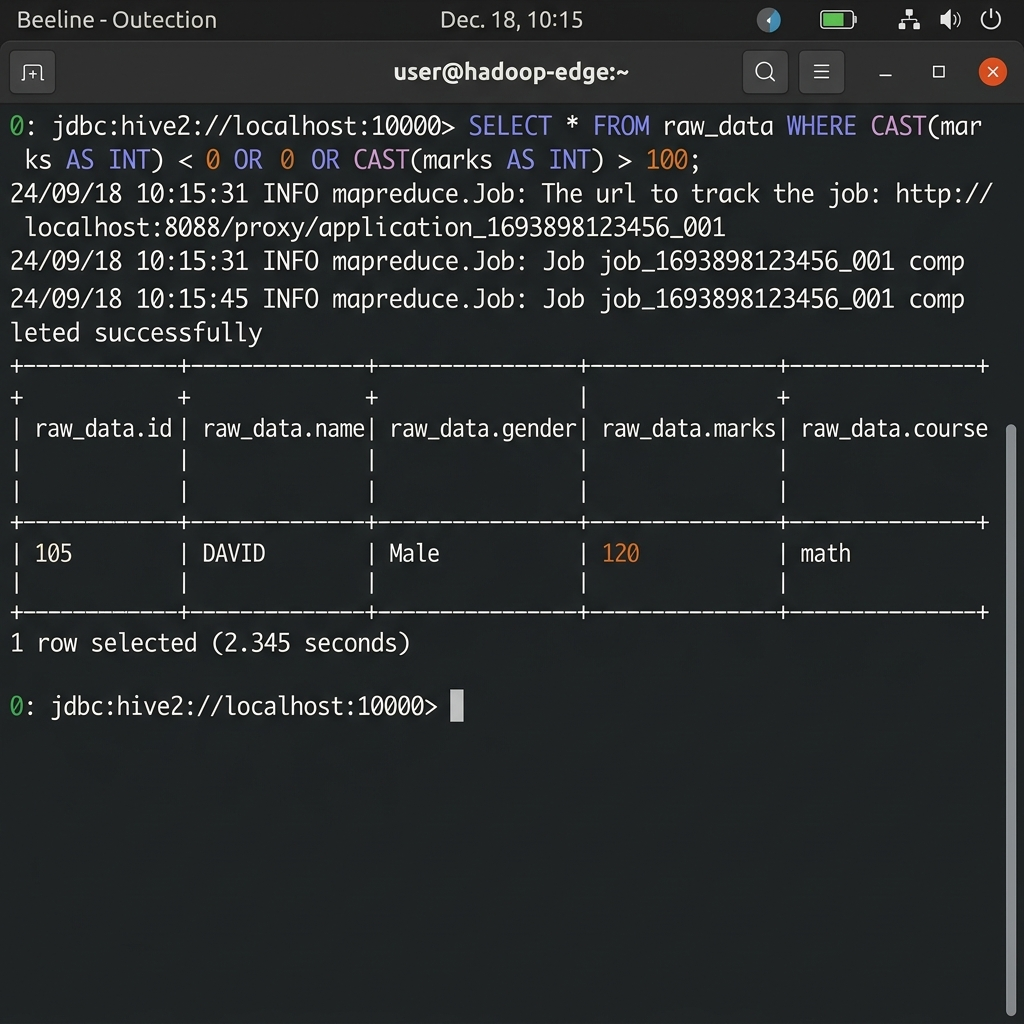
\includegraphics[width=0.95\textwidth]{images/outliers.png}
\caption{Noisy Data/Outliers detected in the staging dataset, filtering out David's out-of-bound score.}
\label{fig:outliers}
\end{figure}

\subsection{Step 7: Final Cleaned Table Creation}
We aggregate all cleaning filters into a CTAS query to create \texttt{cleaned\_student\_scores} in ORC format with Snappy compression:
\begin{lstlisting}[language=SQL]
CREATE TABLE cleaned_student_scores
STORED AS ORC
TBLPROPERTIES ("orc.compress"="SNAPPY") AS
SELECT 
    id,
    UPPER(name) AS name,
    CASE
        WHEN LOWER(gender) IN ('m', 'male') THEN 'Male'
        WHEN LOWER(gender) IN ('f', 'female') THEN 'Female'
        ELSE 'Unknown'
    END AS gender,
    CAST(COALESCE(NULLIF(marks, ''), '0') AS INT) AS marks,
    LOWER(course) AS course
FROM (
    SELECT DISTINCT id, name, gender, marks, course FROM raw_data
) unique_rows
WHERE marks = '' OR (CAST(marks AS INT) BETWEEN 0 AND 100);
\end{lstlisting}

\newpage
\section{Final Execution Results}

\subsection{Memory Tuning for Local Mode}
Running the MapReduce job inside a local, resource-capped JVM (capped at 256MB) triggered \texttt{OutOfMemoryError: Java heap space} due to the Map task sort buffer size (default 100MB). We set the sort buffer to 10MB to resolve this:
\begin{lstlisting}[language=SQL]
SET mapreduce.task.io.sort.mb=10;
\end{lstlisting}

\subsection{Cleaned Dataset Output}
The final cleaned dataset shows perfect de-duplication, format standardizations, and noise removal:

% --- FIGURE 5: FINAL CLEANED DATASET ---
\begin{figure}[H]
\centering
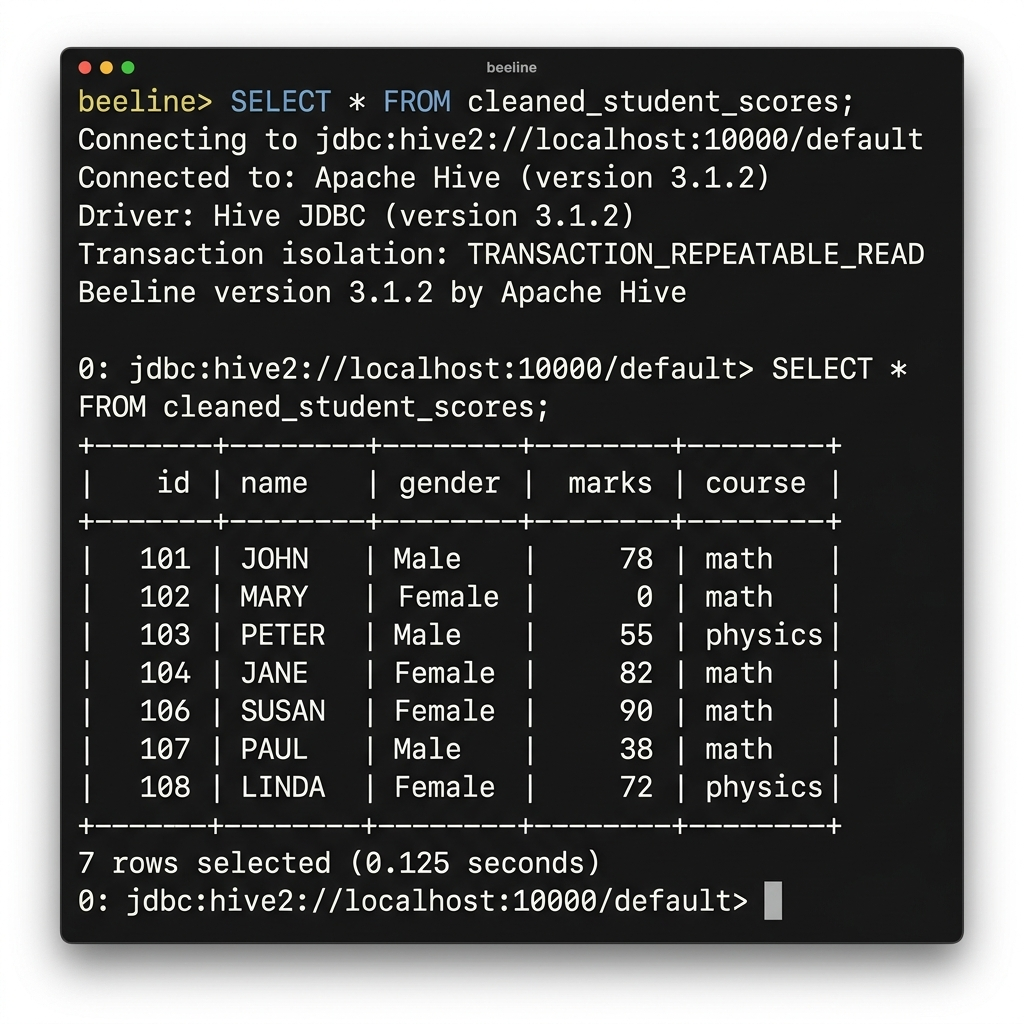
\includegraphics[width=0.95\textwidth]{images/finaldataset.png}
\caption{Final Processed Dataset stored in Hive ORC Table containing 7 cleaned records.}
\label{fig:finaldataset}
\end{figure}

\section{Conclusion}
This lab successfully demonstrates data cleaning and preprocessing inside Apache Hive. By leveraging HQL functions like \texttt{COALESCE}, \texttt{NULLIF}, \texttt{DISTINCT}, and \texttt{CASE} conditional expressions, we transformed raw Excel data into a cleaned table, ready for analytical queries and machine learning models.

\end{document}
